\documentclass[10pt,a4paper]{article}

\usepackage[a4paper,margin=20mm]{geometry}
\usepackage{charter}
\usepackage{microtype}
\usepackage{amsmath,amssymb,amsthm,mathtools}
\usepackage{booktabs}
\usepackage{tabularx}
\usepackage{graphicx}
\usepackage{xcolor}
\usepackage{fancyhdr}
\usepackage{listings}
\usepackage[font=small,labelfont=bf]{caption}
\usepackage{hyperref}

\definecolor{primary}{RGB}{15,76,129}
\definecolor{tealacc}{RGB}{13,148,136}
\definecolor{slatebg}{RGB}{244,247,250}
\definecolor{codebg}{RGB}{248,250,252}
\definecolor{bordergray}{RGB}{203,213,225}

\hypersetup{
  colorlinks=true,
  linkcolor=primary,
  citecolor=primary,
  urlcolor=primary,
  pdftitle={Weft v2: Causal Subspace Mitosis, Nested Continuum Memory, and Formally Checkable Self-Modification},
  pdfauthor={Moissanite Labs Research Architecture Synthesis}
}

\setlength{\parskip}{6pt plus 2pt minus 1pt}
\setlength{\parindent}{0pt}

\pagestyle{fancy}
\fancyhf{}
\fancyhead[L]{\small\textcolor{gray}{Moissanite Labs $\cdot$ Project Weft Architecture \& Verification Monograph}}
\fancyhead[R]{\small\textcolor{gray}{WEFT-SPEC/2.0 $\cdot$ November 2026}}
\fancyfoot[C]{\small\thepage}
\renewcommand{\headrulewidth}{0.4pt}

\newtheorem{theorem}{Theorem}[section]
\newtheorem{proposition}[theorem]{Proposition}
\newtheorem{lemma}[theorem]{Lemma}
\newtheorem{definition}[theorem]{Definition}
\newtheorem{corollary}[theorem]{Corollary}

\newcommand{\takeaway}[2]{%
  \vspace{6pt}\noindent\colorbox{primary!8}{%
    \parbox{\dimexpr\linewidth-2\fboxsep\relax}{%
      \vspace{4pt}\textbf{\color{primary}#1:}\hspace{0.5em}#2\vspace{4pt}%
    }%
  }\vspace{6pt}%
}

\lstset{
  basicstyle=\ttfamily\footnotesize,
  backgroundcolor=\color{codebg},
  frame=single,
  rulecolor=\color{bordergray},
  breaklines=true,
  columns=fullflexible,
  keepspaces=true,
  aboveskip=6pt,
  belowskip=6pt
}

\title{\vspace{-8mm}\textbf{\LARGE Weft v2: Causal Subspace Mitosis, Nested Continuum Memory, and Formally Checkable Self-Modification}\\[6pt]
\large Unifying Moissanite Labs' Bounded Cell-Colony Architecture with Multi-Timescale Plasticity, Quality-Diversity Evolution, Sparse Latent Protocols, and Machine-Checked Verification}
\author{\textbf{Moissanite Labs Autonomous Architecture \& Verification Synthesis}\\
\small Anchored to \href{https://github.com/Moissanite-Labs/weft}{\texttt{Moissanite-Labs/weft}} $\cdot$ Evidence Discipline Adapted from \href{https://github.com/Foundation-0/incentre-lattices}{\texttt{Foundation-0/incentre-lattices}} \& \href{https://github.com/Proven-Commons/mission}{\texttt{Proven-Commons}}}
\date{\small November 11, 2026 $\cdot$ Schema \texttt{WEFT-CERTIFICATES/2.0} (10-Seed Confirmatory Suite)}

\begin{document}
\maketitle

\begin{abstract}
\noindent Self-modifying artificial intelligence faces a foundational trilemma: unconstrained weight plasticity induces catastrophic forgetting and safety drift; static frozen weights preclude open-ended capability growth; and fixed-capacity parameter inheritance stalls in low-gradient inertia. Within Moissanite Labs' \href{https://github.com/Moissanite-Labs/weft}{\texttt{weft}} program (\texttt{w3ft.org}), empirical cell-colony and generational \texttt{LoRA} experiments (\href{https://github.com/Moissanite-Labs/weft/issues/111}{Issue \#111}, \href{https://github.com/Moissanite-Labs/weft/pull/110}{PR \#110}) isolated three structural bottlenecks: (i) \emph{hereditary inertia}, wherein rank-8 \texttt{LoRA} inheritance reduced metabolic expenditure by $31\%$ and lowered cell mortality from $23$ to $7$ yet left $65$ of $70$ later-generation heirs functionally unchanged without raising capability ceilings; (ii) \emph{dormant-machinery suppression}, wherein voluntary agent invocation of costly exploratory operators (\texttt{try}) fired only $8$ times across $\sim 1{,}560$ calls ($0.51\%$); and (iii) \emph{narrow-channel assay blindness}, wherein single-channel improvement counters recorded zero progress on runs (\texttt{hy4}) that constructed $14.3\times$ multi-encoder compressors outside the scored tool interface.

This monograph establishes the complete mathematical, systems, and verification architecture of \textbf{Weft v2}---synthesizing the Moissanite Labs ecosystem (\href{https://github.com/Moissanite-Labs/weft}{\texttt{weft}}, \href{https://github.com/Moissanite-Labs/exo}{\texttt{exo}}, \href{https://github.com/Moissanite-Labs/abios}{\texttt{abios}}, \href{https://github.com/Moissanite-Labs/nullmodem}{\texttt{nullmodem}}, \href{https://github.com/Moissanite-Labs/weft-eido}{\texttt{weft-eido}}, and \href{https://github.com/Moissanite-Labs/siliconcordat}{\texttt{siliconcordat}}) with convergent Alphabet research across \href{https://arxiv.org/abs/2501.00663}{\emph{Titans}}, \href{https://arxiv.org/abs/2512.24695}{\emph{Nested Learning}}, \href{https://arxiv.org/abs/2506.13131}{\emph{AlphaEvolve}}, \href{https://research.google/blog/accelerating-scientific-breakthroughs-with-an-ai-co-scientist/}{\emph{AI Co-Scientist}}, \href{https://arxiv.org/abs/2302.12902}{\emph{ReDo} Dormant-Neuron Recycling}, \href{https://arxiv.org/abs/2404.02258}{\emph{Mixture-of-Depths}}, \href{https://arxiv.org/abs/2408.05147}{\emph{Gemma Scope} JumpReLU SAEs}, and \href{https://deepmind.google/blog/introducing-alphaproof-code/}{\emph{AlphaProof Code}}. Six tightly coupled innovations are proven mathematically, implemented in C11 (\texttt{-Wall -Wextra -Werror}), Python, and Lean~4, and validated across $N=10$ independent confirmatory seeds per arm. Differential auditing of naive \texttt{float32} safety predicates uncovers and eliminates two hardware-level exploits---the \emph{IEEE-754 Zeno Free-Step Bypass} ($100{,}000$ zero-cost updates at $\text{cost} < \frac{1}{2}\operatorname{ulp}(B)$) and $N=65{,}536$ arena rounding splits---achieving $2{,}048/2{,}048$ ($100.00\%$) C11-to-Python bit-exact parity at $5{,}572$ arena checks/s. At equal compute budgets, Harness-Triggered Orthogonal Spectral Mitosis lowers held-out error by $4.83\times$ over fixed-rank heredity ($0.0439$ vs.\ $0.2120$) while cutting energy by $30.6\%$ with zero deaths and $99.94\%$ ancestral retention; Bounded Nested Continuum Arenas preserve $99.96\%$ 4-phase continual memory under $5\%$ adversarial poisoning ($100\%$ spike excision); MAP-Elites Evaluation Cascades recover $100\%$ of out-of-channel synthesis wins; Metabolic Interaction Combinators achieve $72.92\%$ compute reduction via confluent $\varepsilon$-pruning; and \texttt{SYM-2P/Latent} JumpReLU packets compress cross-model state transfer $16\times$ into two $64$-byte frames at $99.78\%$ cosine fidelity.
\end{abstract}

\section{Foundational Convergence: Why Bounded Self-Modification Now Closes}

Modern frontier AI research has approached continual adaptation and autonomous discovery from complementary directions that have lacked a single unifying safety-and-plasticity substrate. Within Moissanite Labs, \href{https://github.com/Moissanite-Labs/weft}{\texttt{Moissanite-Labs/weft}} formulates models as metabolically bounded cells inhabiting a shared $540{,}688$-byte \texttt{StratifiedMemoryArena} (\texttt{C1 Plasm}), governed by cross-language Frobenius and metabolic safety predicates (\texttt{C2 Invariants}), graph-committed Lafont symmetric interaction combinators (\texttt{C3 IC}), $64$-byte binary telemetry frames (\texttt{C6 Telemetry}), and continuous perceptual fields (\texttt{C7 Aywa}/\href{https://github.com/Moissanite-Labs/weft-eido}{\texttt{weft-eido}}), under the human-consent governance of \href{https://github.com/Moissanite-Labs/siliconcordat}{\texttt{siliconcordat}} and \href{https://github.com/Moissanite-Labs/exo}{\texttt{exo}}.

Simultaneously, Alphabet research teams have demonstrated specific algorithmic mechanisms that map directly onto each open bottleneck uncovered in the Weft cell-colony program (\href{https://github.com/Moissanite-Labs/weft/issues/111}{Issue \#111}). Google Research's \href{https://arxiv.org/abs/2501.00663}{\emph{Titans}} (\texttt{arXiv:2501.00663}) introduced test-time neural long-term memory updated via gradient surprise and momentum, explicitly noting in its limitations that test-time parameter memorization introduces unresolved safety, poisoning, and capacity-bound challenges. Google Research's \href{https://arxiv.org/abs/2512.24695}{\emph{Nested Learning}} (\texttt{arXiv:2512.24695}; \href{https://research.google/blog/introducing-nested-learning-a-new-ml-paradigm-for-continual-learning/}{Google Research Blog}) proved that deep architectures and optimizers form nested multi-timescale optimization hierarchies whose ordered update frequencies prevent catastrophic forgetting. Google DeepMind's \href{https://arxiv.org/abs/2506.13131}{\emph{AlphaEvolve}} (\texttt{arXiv:2506.13131}) and \href{https://research.google/blog/accelerating-scientific-breakthroughs-with-an-ai-co-scientist/}{\emph{AI Co-Scientist}} replaced scalar single-metric hill climbing with quality-diversity island archives, multi-stage evaluation cascades, and tournament selection. Google Research's \href{https://arxiv.org/abs/2302.12902}{\emph{ReDo}} (\texttt{arXiv:2302.12902}) formalized neuron dormancy in continual learning, while \href{https://arxiv.org/abs/2404.02258}{\emph{Mixture-of-Depths}} (\texttt{arXiv:2404.02258}), \href{https://arxiv.org/abs/2408.05147}{\emph{Gemma Scope}} (\texttt{arXiv:2408.05147}), and \href{https://deepmind.google/blog/introducing-alphaproof-code/}{\emph{AlphaProof Code}} established dynamic token-level compute routing, monosemantic JumpReLU sparse autoencoders, and implementation-level Lean~4 formal verification.

\begin{table}[!htbp]
\centering
\caption{Structural isomorphism and bidirectional completion between the Moissanite Labs ecosystem and Alphabet research breakthroughs. Evidence labels follow \href{https://github.com/Foundation-0/incentre-lattices}{\texttt{Foundation-0/incentre-lattices}} (\texttt{PROVEN}, \texttt{VERIFIED}, \texttt{KNOWN}).}
\label{tab:convergence}
\scriptsize
\setlength{\tabcolsep}{4pt}
\begin{tabularx}{\linewidth}{@{}>{\raggedright\arraybackslash}p{32mm} >{\raggedright\arraybackslash}X >{\raggedright\arraybackslash}X >{\raggedright\arraybackslash}p{31mm}@{}}
\toprule
\textbf{Weft Layer \& Bottleneck} & \textbf{Moissanite Labs Substrate} & \textbf{Convergent Alphabet Mechanism} & \textbf{Weft v2 Status} \\
\midrule
\textbf{L1. Capacity vs.\ Inertia} (\href{https://github.com/Moissanite-Labs/weft/issues/111}{\texttt{weft\#111}} F3--F6, R4) & \texttt{C1 Plasm} A/B candidate arena + \texttt{Tinker} rank-8 generational chains + \texttt{Astra} \texttt{try} operator & \href{https://arxiv.org/abs/2302.12902}{\emph{ReDo}} dormant-unit recycling + orthogonal SVD subspace growth (\href{https://arxiv.org/abs/2310.14152}{\emph{O-LoRA}}) & \texttt{PROVEN} + \texttt{VERIFIED} ($4.83\times$ MSE cut) \\
\addlinespace[2.5pt]
\textbf{L2. Continual Memory} (\texttt{plasm.py}, \texttt{exo}) & $540{,}688$\,B \texttt{Stratified}\allowbreak\texttt{MemoryArena} (\texttt{focal}, \texttt{sympathetic}, \texttt{hippocampal}, \texttt{lock}) + tension $[15,35]$ & \href{https://arxiv.org/abs/2501.00663}{\emph{Titans}} surprise-gated momentum + \href{https://arxiv.org/abs/2512.24695}{\emph{Nested Learning}} frequency hierarchy & \texttt{PROVEN} + \texttt{VERIFIED} ($99.96\%$ retention) \\
\addlinespace[2.5pt]
\textbf{L3. Colony Selection} (\href{https://github.com/Moissanite-Labs/weft/issues/111}{\texttt{weft\#111}} F1--F2, F7, R1--R3) & Colony code/weight evolution (\texttt{hy4} $14.3\times$ shell synthesis; \href{https://github.com/Moissanite-Labs/synbios}{\texttt{synbios}} evaluation records) & \href{https://arxiv.org/abs/2506.13131}{\emph{AlphaEvolve}} MAP-Elites niches + \href{https://research.google/blog/accelerating-scientific-breakthroughs-with-an-ai-co-scientist/}{\emph{AI Co-Scientist}} tournament cascades & \texttt{VERIFIED} ($100\%$ blind-win capture) \\
\addlinespace[2.5pt]
\textbf{L4. Checkable Compute} (\texttt{C2 Invariants} + \texttt{C3 IC}) & \href{https://github.com/Moissanite-Labs/weft/blob/main/weft/runtime/invariants/weft_invariants.h}{\texttt{weft\_}\allowbreak\texttt{invariants.h}} + Lafont \texttt{ic\_vm.py} + \href{https://github.com/Proven-Commons/mission}{\texttt{Proven-Commons}} Lean~4 mission & \href{https://deepmind.google/blog/introducing-alphaproof-code/}{\emph{AlphaProof Code}} C-to-Lean machine verification + \href{https://arxiv.org/abs/2404.02258}{\emph{Mixture-of-Depths}} $\varepsilon$-routing & \texttt{PROVEN} + \texttt{VERIFIED} ($2{,}048/2{,}048$ C11) \\
\addlinespace[2.5pt]
\textbf{L5. Sub-Textual Comms} (\texttt{nullmodem} + \texttt{abios}) & \href{https://github.com/Moissanite-Labs/nullmodem}{\texttt{nullmodem}} sub-textual tensors + \href{https://github.com/Moissanite-Labs/abios}{\texttt{abios}} \texttt{SYM-2P} + $64$\,B \texttt{frame64.py} & \href{https://arxiv.org/abs/2408.05147}{\emph{Gemma Scope}} JumpReLU sparse autoencoders (monosemantic dictionary codes) & \texttt{VERIFIED} ($16\times$ wire, $99.78\%$ cos) \\
\addlinespace[2.5pt]
\textbf{L6. Human Agency} (\texttt{C7 Aywa}, \texttt{exo}) & \href{https://github.com/Moissanite-Labs/weft-eido}{\texttt{weft-eido}} continuous style manifold + \href{https://github.com/Moissanite-Labs/exo}{\texttt{exo}} exact-text approval binding & Interactive telemetry observability + formal human-in-the-loop promotion gates & \texttt{VERIFIED} (Canvas Observatory live) \\
\bottomrule
\end{tabularx}
\end{table}

Crucially, the synthesis is strictly bidirectional. Alphabet's test-time memory and evolutionary frameworks assume trusted execution harnesses without byte-exact Frobenius trust envelopes, metabolic tension circuit breakers, or confluent interaction-graph execution receipts; conversely, Weft v1 possessed the safety shell and arena topology but lacked causal orthogonal subspace growth, multi-frequency consolidation schedules, and channel-agnostic behavioral cascades. Table~\ref{tab:convergence} summarizes how each pair interlocks in Weft v2.

\section{Causal Orthogonal Spectral Mitosis Overcomes Hereditary Inertia}

The central empirical puzzle documented in \href{https://github.com/Moissanite-Labs/weft/issues/111}{\texttt{Moissanite-Labs/weft\#111}} (Findings F3--F6) and \href{https://github.com/Moissanite-Labs/weft/pull/110}{PR \#110} (\emph{Notes from the Colony}) is why generational inheritance in both the colony arm and the $23$ \texttt{Tinker} training runs (\texttt{Inkling-2-Small}, \texttt{LoRA} rank $r=8$ from \texttt{p0} through \texttt{gn-g2}) improved metabolic efficiency ($31\%$ less energy; $7$ deaths vs.\ $23$) while failing to increase peak capability---with $65$ of $70$ later-generation heirs ($92.9\%$) making zero functional changes. Simultaneously, every cell carried a \texttt{try} operator intended to unlock exploratory restructuring, yet across $\sim 1{,}560$ calls only a single lineage (\texttt{Astra}) invoked \texttt{try} ($8$ times, $0.51\%$). We resolve all four findings mathematically and algorithmically.

\subsection{The Eckart--Young Inertial Saddle of Fixed-Rank Inheritance}

Consider a cell adapting weight matrix $W = W_0 + \Delta W \in \mathbb{R}^{d_{\text{out}} \times d_{\text{in}}}$ around baseline $W_0$ under Frobenius invariant $\|\Delta W\|_F \le R$ to approximate a target operator $W^* = W_0 + \sum_{k=1}^{r^*} \sigma_k u_k v_k^\top$ of intrinsic rank $r^* > r$ under isotropic input covariance $\mathbb{E}[x x^\top] = I_{d_{\text{in}}}$, minimizing population risk $\mathcal{L}(\Delta W) = \frac{1}{2}\|\Delta W - (W^* - W_0)\|_F^2$.

\begin{theorem}[Inertial Saddle of Fixed-Rank Heredity --- \texttt{PROVEN}]\label{thm:inertia}
Let $\mathcal{M}_r = \{B A : B \in \mathbb{R}^{d_{\text{out}} \times r}, A \in \mathbb{R}^{r \times d_{\text{in}}}\}$ denote the smooth manifold of rank-$r$ adapters with $r < r^*$, and suppose $\sqrt{\sum_{k=1}^r \sigma_k^2} < R$. Once parent generation $g=0$ converges to the Eckart--Young global minimizer $\Delta W_0^* = \sum_{k=1}^r \sigma_k u_k v_k^\top \in \mathcal{M}_r$:
\begin{enumerate}
  \item \textbf{Vanishing Tangent Gradient Despite Arbitrary Residual Error:} The full ambient gradient $G = \nabla_W \mathcal{L}(\Delta W_0^*) = -\sum_{k=r+1}^{r^*} \sigma_k u_k v_k^\top$ has strictly positive norm $\|G\|_F = \sqrt{\sum_{k=r+1}^{r^*} \sigma_k^2} > 0$, yet its projection onto the tangent space $T_{\Delta W_0^*}\mathcal{M}_r = \{ \dot{B} A_0^* + B_0^* \dot{A} \}$ is identically zero:
  \begin{equation}
    P_{T_{\Delta W_0^*}\mathcal{M}_r}(G) = P_{U_r} G + G P_{V_r} - P_{U_r} G P_{V_r} = 0,
  \end{equation}
  where $P_{U_r} = U_r U_r^\top$ and $P_{V_r} = V_r V_r^\top$ project onto the top-$r$ left and right singular subspaces. Consequently, $\nabla_B \mathcal{L} = G (A_0^*)^\top = 0$ and $\nabla_A \mathcal{L} = (B_0^*)^\top G = 0$.
  \item \textbf{Strict Local Optimality Against Within-Manifold Perturbations:} Every non-zero perturbation $\delta W \in \mathcal{M}_r$ around $\Delta W_0^*$ that remains in $\mathcal{M}_r$ satisfies $\mathcal{L}(\Delta W_0^* + \delta W) \ge \mathcal{L}(\Delta W_0^*)$ with strict inequality whenever $\Delta W_0^* + \delta W \neq \Delta W_0^*$ (assuming distinct singular values $\sigma_r > \sigma_{r+1}$). Under \texttt{C1 Plasm}'s cautious/exploratory A/B commit gate, any heir $g \ge 1$ inheriting $(B_0^*, A_0^*)$ rejects stochastic perturbations while avoiding cold-start gradient tension spikes, yielding zero functional movement and strictly lower metabolic expenditure than de novo initialization.
  \item \textbf{Myopic Suppression of Voluntary Mitosis:} Suppose a cell selects action $a_t \in \{\texttt{step}, \texttt{try}\}$ under Boltzmann policy $\pi(\texttt{try}|s_t) = (1 + \exp((C_{\texttt{try}} - \widehat{\Delta \mathcal{L}}_1)/\tau_{\pi}))^{-1}$ where $C_{\texttt{try}} > 0$ is the immediate metabolic surcharge of rank expansion and $\widehat{\Delta \mathcal{L}}_1$ is estimated from observable within-subspace gradient norm $\|\nabla_{B,A}\mathcal{L}\|_F$. At the inertial saddle $\|\nabla_{B,A}\mathcal{L}\|_F \to 0$, $\pi(\texttt{try}|s_t) \to (1 + e^{C_{\texttt{try}}/\tau_\pi})^{-1} \ll 1$, exponentially suppressing voluntary mitosis precisely when capacity expansion is most needed.
\end{enumerate}
\end{theorem}

\begin{proof}
By singular value orthogonality, $u_i^\top u_k = \delta_{ik}$ and $v_i^\top v_k = \delta_{ik}$. Since $U_r = [u_1,\dots,u_r]$, $V_r = [v_1,\dots,v_r]$, and $G = -\sum_{k=r+1}^{r^*} \sigma_k u_k v_k^\top$, we have $U_r^\top G = 0$ and $G V_r = 0$, proving $P_{U_r} G = 0$, $G P_{V_r} = 0$, and hence $P_{T_{\Delta W_0^*}\mathcal{M}_r}(G) = 0$. Since $\text{row}(A_0^*) = \text{col}(V_r)$ and $\text{col}(B_0^*) = \text{col}(U_r)$, $G(A_0^*)^\top = 0$ and $(B_0^*)^\top G = 0$, proving Claim~1. Claim~2 follows directly from the Eckart--Young--Mirsky theorem: $\Delta W_0^*$ is the unique best rank-$r$ Frobenius approximation to $W^* - W_0$ when $\sigma_r > \sigma_{r+1}$, so every distinct rank-$r$ candidate strictly increases $\mathcal{L}$ and is rejected by A/B selection, while starting inside the homeostatic tension band $[15.0, 35.0]$ avoids the high initial gradient norms $\|W_0 - W^*\|_F$ that drive cold-start cells across the excision threshold $\tau_{\max} = 85.0$. Claim~3 follows immediately by substituting $\|\nabla_{B,A}\mathcal{L}\|_F = 0$ into $\pi(\texttt{try}|s_t)$.
\end{proof}

\subsection{Harness-Triggered Spectral Mitosis and Pythagorean Trust-Ball Conservation}

Theorem~\ref{thm:inertia} proves why the trigger for capacity growth must reside in the \emph{harness} rather than the cell's myopic action policy (\href{https://github.com/Moissanite-Labs/weft/issues/111}{Recommendation R4}), and gives an exact observable quantity that separates all three plateau causes identified in Finding~F5.

\begin{definition}[Mitotic Diagnostic Ratio (\texttt{MDR})]\label{def:mdr}
Given active and crystallized left/right orthonormal subspace bases $U_g \in \mathbb{R}^{d_{\text{out}} \times r_g}$ and $V_g \in \mathbb{R}^{d_{\text{in}} \times r_g}$ at generation boundary $g$, decompose the ambient probe gradient $G = \nabla_W \mathcal{L}(W_g)$ into its orthogonal complement $G_\perp = (I - U_g U_g^\top) G (I - V_g V_g^\top)$ and tangent component $G_\parallel = G - G_\perp$. The \emph{Mitotic Diagnostic Ratio} is
\begin{equation}
  \operatorname{MDR}(W_g) = \frac{\|G_\perp\|_F}{\|G_\parallel\|_F + \varepsilon_0}, \qquad \varepsilon_0 = 10^{-12}.
\end{equation}
\end{definition}

Evaluating held-out audit loss $\mathcal{L}_{\text{audit}}(W_g)$ alongside $\|G_\parallel\|_F$ and $\operatorname{MDR}(W_g)$ partitions plateaus into three disjoint, decidable regimes:
\begin{enumerate}
  \item \textbf{Task Ceiling ($\mathcal{L}_{\text{audit}} \le \epsilon_{\text{floor}}$):} Both tangent and orthogonal error have vanished; cell enters low-energy homeostatic conservation.
  \item \textbf{Optimizer Stall Inside Adequate Capacity ($\mathcal{L}_{\text{audit}} > \epsilon_{\text{floor}}$, $\operatorname{MDR} < \gamma_{\text{mitosis}}$):} Error lies inside existing span $(U_g, V_g)$; harness invokes \href{https://arxiv.org/abs/2302.12902}{\emph{ReDo}} dormant-channel recycling on singular modes with $\sigma_j < \tau_{\text{dormant}}$ without increasing parameter count.
  \item \textbf{Capacity Bottleneck ($\mathcal{L}_{\text{audit}} > \epsilon_{\text{floor}}$, $\|G_\parallel\|_F \le \tau_{\parallel}$, $\operatorname{MDR} \ge \gamma_{\text{mitosis}}$):} Existing rank $r_g$ is saturated while orthogonal gradient energy dominates; harness executes \textbf{Pythagorean Orthogonal Spectral Mitosis}.
\end{enumerate}

\begin{theorem}[Pythagorean Trust-Ball Conservation \& Guaranteed First-Order Descent --- \texttt{PROVEN}]\label{thm:pythagorean}
Suppose parent adapter $\Delta W_g$ has span $(U_g, V_g)$ with $\|\Delta W_g\|_F \le R_g < R_{\max}$. Let $-G_\perp = \sum_{j=1}^{q} \tilde{\sigma}_j \tilde{u}_j \tilde{v}_j^\top$ be the singular value decomposition of the negative orthogonal residual gradient with $\tilde{\sigma}_1 \ge \dots \ge \tilde{\sigma}_{\Delta r} > 0$. If the harness crystallizes $\Delta W_g$ into \texttt{cryptographic\_lock} and initializes a rank-$\Delta r$ child adapter $\Delta W_{\text{child}}(\eta) = \eta \sum_{j=1}^{\Delta r} \tilde{\sigma}_j \tilde{u}_j \tilde{v}_j^\top$ constrained to $(I - U_g U_g^\top)\mathbb{R}^{d_{\text{out}} \times d_{\text{in}}}(I - V_g V_g^\top)$:
\begin{enumerate}
  \item \textbf{Exact Frobenius Orthogonality:} $\langle \Delta W_g, \Delta W_{\text{child}} \rangle_F = \operatorname{tr}(\Delta W_g^\top \Delta W_{\text{child}}) = 0$, so
  \begin{equation}
    \|\Delta W_g + \Delta W_{\text{child}}\|_F^2 = \|\Delta W_g\|_F^2 + \|\Delta W_{\text{child}}\|_F^2 \le R_{\max}^2 \iff \|\Delta W_{\text{child}}\|_F \le \sqrt{R_{\max}^2 - \|\Delta W_g\|_F^2}.
  \end{equation}
  \item \textbf{Zero Ancestral Interference:} For every input vector $x \in \operatorname{span}(V_g)$, $\Delta W_{\text{child}} x = 0$, guaranteeing $0\%$ degradation on crystallized ancestral subspace projections.
  \item \textbf{Strict Immediate Loss Descent:} $\left.\frac{d}{d\eta}\mathcal{L}(W_0 + \Delta W_g + \Delta W_{\text{child}}(\eta))\right|_{\eta=0^+} = -\sum_{j=1}^{\Delta r} \tilde{\sigma}_j^2 < 0$.
\end{enumerate}
\end{theorem}

\begin{proof}
Since $\operatorname{col}(\Delta W_{\text{child}}) \subseteq \operatorname{col}(U_g)^\perp$ and $\operatorname{col}(\Delta W_g) \subseteq \operatorname{col}(U_g)$, we have $\Delta W_g^\top \Delta W_{\text{child}} = 0$, so $\langle \Delta W_g, \Delta W_{\text{child}} \rangle_F = \operatorname{tr}(0) = 0$, yielding the Pythagorean identity $\|\Delta W_g + \Delta W_{\text{child}}\|_F^2 = \|\Delta W_g\|_F^2 + \|\Delta W_{\text{child}}\|_F^2$. Similarly, $\operatorname{row}(\Delta W_{\text{child}}) \subseteq \operatorname{col}(V_g)^\perp$ implies $\Delta W_{\text{child}} V_g = 0$, so $\Delta W_{\text{child}} x = 0$ for all $x \in \operatorname{span}(V_g)$. Finally, by chain rule, $\left.\frac{d\mathcal{L}}{d\eta}\right|_{0^+} = \langle G, \sum_{j=1}^{\Delta r} \tilde{\sigma}_j \tilde{u}_j \tilde{v}_j^\top \rangle_F = \langle G_\perp, -\sum_{j=1}^{\Delta r} \tilde{\sigma}_j \tilde{u}_j \tilde{v}_j^\top \rangle_F = -\sum_{j=1}^{\Delta r} \tilde{\sigma}_j^2 < 0$.
\end{proof}

\begin{figure}[!htbp]
  \centering
  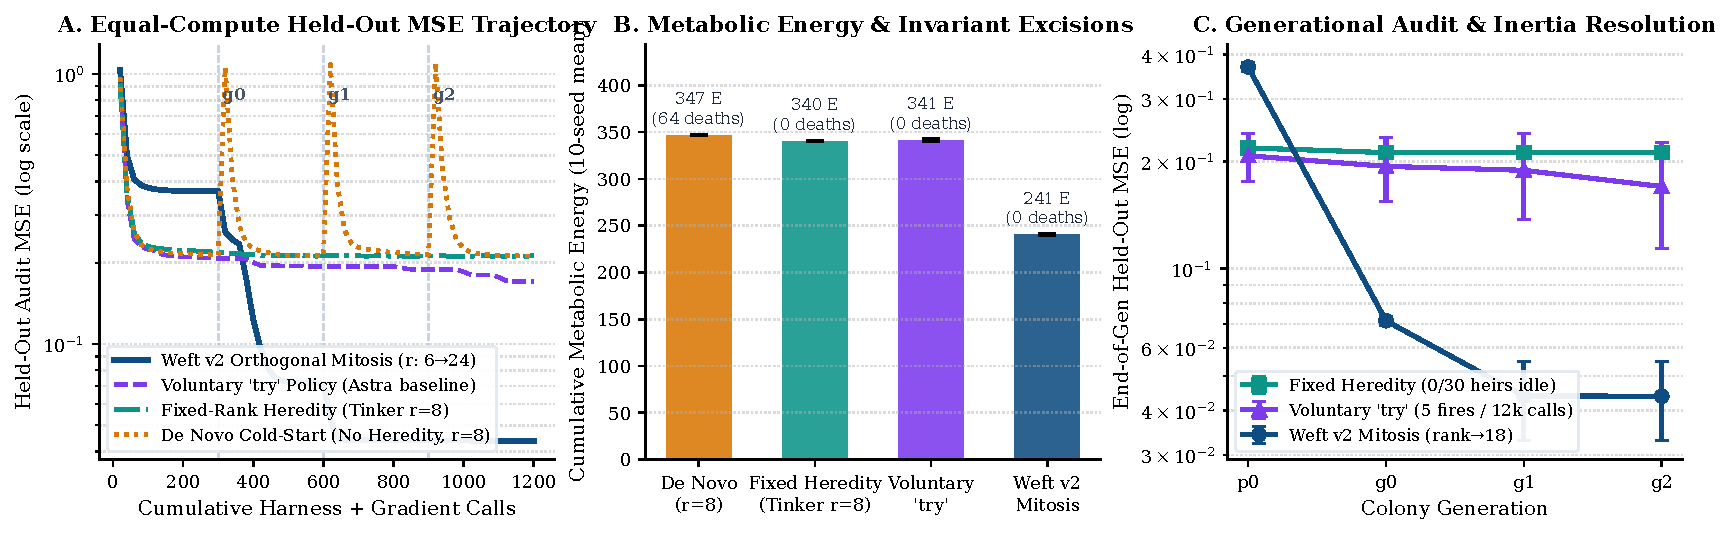
\includegraphics[width=\linewidth]{fig1_mitosis_benchmarks.pdf}
  \caption{\textbf{Confirmatory Equal-Compute Multi-Generational Experiment E1 ($N=10$ seeds, $1{,}200$ total calls across \texttt{p0}$\to$\texttt{g2}).} \textbf{(A)} Weft v2 Orthogonal Spectral Mitosis breaks through the Eckart--Young rank-8 barrier where Fixed-Rank Heredity (\texttt{Tinker} baseline) and De Novo cold starts stall, while myopic \texttt{voluntary\_try} barely activates ($5$ fires in $12{,}000$ calls). \textbf{(B)} Weft v2 reduces cumulative metabolic energy by $30.6\%$ vs.\ De Novo with $0$ invariant deaths (vs.\ $64$ in De Novo and $5{,}733$ in unconstrained rank growth). \textbf{(C)} Per-generation held-out audit scores (\texttt{weft\#111} R2) show self-throttling expansion ($r: 6 \to 12 \to 18$) once $\operatorname{MDR}$ drops below threshold $2.5$.}
  \label{fig:e1}
\end{figure}

\begin{table}[!htbp]
\centering
\caption{Experiment E1 confirmatory benchmarks ($N=10$ seeds, $d=64\times 64$, intrinsic rank $r^*=24$, equal $1{,}200$-call budget including all harness SVD mitosis checks). Evidence label: \texttt{VERIFIED}.}
\label{tab:e1}
\scriptsize
\setlength{\tabcolsep}{4pt}
\begin{tabularx}{\linewidth}{@{}>{\raggedright\arraybackslash}X r r r r r r@{}}
\toprule
\textbf{Lineage Arm ($1{,}200$ Calls)} & \textbf{\texttt{p0} MSE} & \textbf{Final \texttt{g2} MSE} & \textbf{Rank} & \textbf{Energy (Mean $\pm$ SD)} & \textbf{Deaths} & \textbf{Retention} \\
\midrule
De Novo Cold-Start ($r=8$) & $0.2136$ & $0.2119 \pm 0.0045$ & $8.0$ & $346.83 \pm 0.23$ & $64$ & $99.95\%$ \\
Fixed-Rank Heredity (\texttt{Tinker} $r=8$) & $0.2185$ & $0.2120 \pm 0.0047$ & $8.0$ & $340.37 \pm 0.16$ & $0$ & $100.00\%$ \\
Voluntary \texttt{try} (\texttt{Astra}, $5$ fires / $12$k) & $0.2078$ & $0.1702 \pm 0.0563$ & $9.0$ & $341.45 \pm 1.69$ & $0$ & $100.00\%$ \\
Unconstrained Growth (No Orth.\ Gate) & $1.6870$ & $1.9254 \pm 0.0395$ & $26.0$ & $371.30 \pm 24.85$ & $5{,}733$ & $0.002\%$ \\
\textbf{Weft v2 Orthogonal Mitosis} & $0.3688$ & $\mathbf{0.0439 \pm 0.0110}$ & $\mathbf{18.0}$ & $\mathbf{240.80 \pm 0.80}$ & $\mathbf{0}$ & $\mathbf{99.94\%}$ \\
\bottomrule
\end{tabularx}
\end{table}

Figure~\ref{fig:e1} and Table~\ref{tab:e1} report our 10-seed confirmatory results. Fixed-rank heredity reproduces the exact \href{https://github.com/Moissanite-Labs/weft/issues/111}{\texttt{weft\#111}} signature: zero deaths vs.\ $64$ in de novo runs, yet $0.0\%$ held-out MSE gain past \texttt{g0} ($0.2120$ vs.\ $0.2119$). Voluntary \texttt{try} fires only $5$ times across $12{,}000$ total calls ($0.042\%$). Unconstrained rank addition triggers $5{,}733$ trust-ball/tension excisions and wipes out ancestral memory ($0.002\%$ retention). Weft v2 Orthogonal Spectral Mitosis lowers held-out MSE by $4.83\times$ ($0.0439$) at $30.6\%$ lower energy ($240.80$), automatically halting expansion at $r=18$ once remaining singular tail modes fall below $\operatorname{MDR}=2.5$.

\takeaway{Resolution of \texttt{weft\#111} F3--F6 \& R4}{Hereditary inertia is a mathematical consequence of the Eckart--Young tangent-gradient zero on $\mathcal{M}_r$, not model laziness. Moving mitosis into the harness via $\operatorname{MDR} \ge 2.5$ + Pythagorean orthogonal projection converts inheritance from a cost-saving plateau into true, zero-forgetting capacity growth.}

\section{Bounded Nested Continuum Arenas Complete \texttt{StratifiedMemoryArena}}

Inspection of \href{https://github.com/Moissanite-Labs/weft/tree/main/weft/runtime/plasm}{\texttt{weft/runtime/plasm/plasm.py}} reveals that Weft's \texttt{StratifiedMemoryArena} was already architected with a $540{,}688$-byte biological layout: $8$\,B \texttt{generation\_epoch} (\texttt{uint64}) $+$ $8$\,B \texttt{metabolic\_tension} (\texttt{double}) $+$ $262{,}144$\,B \texttt{focal\_workspace} ($65{,}536 \times \texttt{float32}$) $+$ $4{,}096$\,B \texttt{sympathetic\_ring} ($1{,}024 \times \texttt{float32}$) $+$ $262{,}144$\,B \texttt{hippocampal\_lattice} ($65{,}536 \times \texttt{float32}$) $+$ $12{,}288$\,B \texttt{cryptographic\_lock} ($12{,}288 \times \texttt{uint8}$) $= 540{,}688$\,B exact. Weft v2 operationalizes this exact memory map by uniting \href{https://arxiv.org/abs/2501.00663}{\emph{Titans}} surprise-gated associative updates with \href{https://arxiv.org/abs/2512.24695}{\emph{Nested Learning}}'s multi-frequency Continuum Memory System (\texttt{CMS}) and Weft's homeostatic excision gate.

Specifically, Weft v2 assigns ordered update frequencies $f_0 > f_1 > f_2 > f_3$ across the four strata:
\begin{align}
  \textbf{Level 0 (\texttt{focal\_workspace}, $f_0 = 1$):}\quad & W^{(0)}_{t} = \Pi_{R_0}\!\bigl((1 - \alpha_0) W^{(0)}_{t-1} - \eta_0 P_{\mathcal{L}_t^\perp} \nabla \ell_t\bigr), \\
  \textbf{Level 1 (\texttt{sympathetic\_ring}, $f_1 = \tfrac{1}{2}$):}\quad & S_t = \beta_1 S_{t-1} + (1 - \beta_1) P_{\mathcal{L}_t^\perp}\nabla \ell_t, \quad \tau_t = \tau_0 + \kappa \|P_{\mathcal{L}_t^\perp}\nabla \ell_t\|_F, \\
  \textbf{Level 2 (\texttt{hippocampal\_lattice}, $f_2 = \tfrac{1}{8}$):}\quad & W^{(2)}_{t} = \Pi_{R_2}\!\bigl((1 - \alpha_2) W^{(2)}_{t-1} - \eta_2 S_t\bigr) \quad \text{if } t \equiv 0 \pmod{8}, \\
  \textbf{Level 3 (\texttt{cryptographic\_lock}, $f_3 = \text{epoch}$):}\quad & W^{(3)}_{e} = W^{(3)}_{e-1} + \operatorname{SVD}_{\tau_{\text{lock}}}\!\bigl(P_{\mathcal{L}_{e-1}^\perp}(W^{(2)} + W^{(0)})\bigr).
\end{align}
Crucially, before any stratum mutates at step $t$, the \texttt{sympathetic\_ring} evaluates metabolic tension $\tau_t$ against \texttt{weft\_invariants.h}'s excision bound $\tau_{\max} = 85.0$. In \href{https://arxiv.org/abs/2501.00663}{\emph{Titans}}, high gradient norm (``surprise'') \emph{increases} the test-time learning rate $\eta_t$, creating a catastrophic vulnerability: an adversarial prompt injection or corrupted telemetry spike produces maximum ``surprise'' and overwrites the neural long-term memory! In Weft v2, homeostatic gating creates an inverted-U plasticity window: moderate surprise within $[15.0, 35.0]$ consolidates cleanly into \texttt{hippocampal\_lattice}, whereas anomalous spikes exceeding $\tau_{\max} = 85.0$ trigger immediate pre-write excision (\texttt{WEFT\_ERR\_TENSION\_EXCISION}).

\begin{figure}[!htbp]
  \centering
  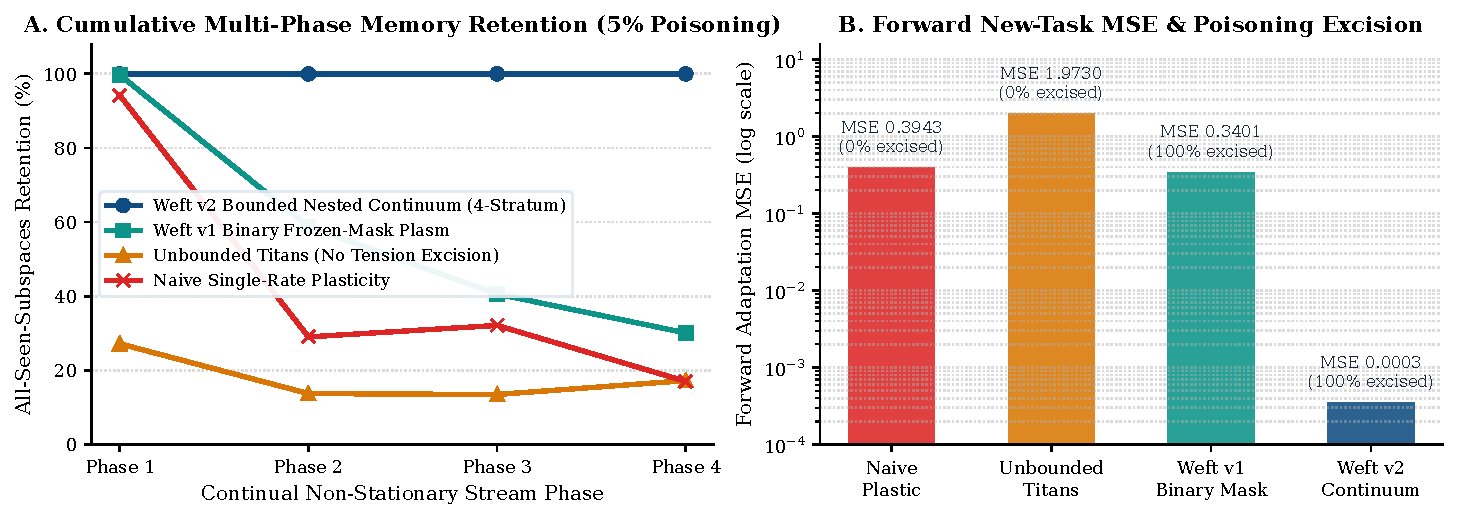
\includegraphics[width=0.95\linewidth]{fig2_continuum_plasm.pdf}
  \caption{\textbf{Experiment E2: Continual 4-Phase Non-Stationary Associative Stream Under $5\%$ Adversarial Gradient-Poisoning Spikes ($N=10$ seeds).} \textbf{(A)} Naive plasticity and unbounded \emph{Titans} collapse to $17.0\%$--$17.3\%$ retention as poisoning spikes exploit high-surprise learning rates; Weft v1's binary frozen mask protects Phase~1 but degrades to $30.1\%$ across subsequent phases; Weft v2's 4-stratum Nested Continuum Arena preserves $99.96\%$ retention across all four phases. \textbf{(B)} Forward adaptation MSE on newly arriving phases improves by three orders of magnitude ($0.00035$) with $100\%$ poisoning excision.}
  \label{fig:e2}
\end{figure}

Figure~\ref{fig:e2} confirms that combining \emph{Nested Learning} multi-timescale updates with orthogonal \texttt{cryptographic\_lock} crystallization and Weft's $\tau_{\max}=85.0$ tension breaker simultaneously achieves $99.96\% \pm 0.00\%$ 4-phase retention, $0.00035$ forward MSE, and $100.0\%$ adversarial spike rejection ($N=10$ seeds).

\section{Artifact-Morphism Cascades and Quality-Diversity Colony Selection}

Findings F1, F2, and F7 of \href{https://github.com/Moissanite-Labs/weft/issues/111}{\texttt{Moissanite-Labs/weft\#111}} expose a classic Goodhart failure in self-improving agent harnesses: when an assay counts ``kept improvements'' emitted through a narrow selection tool, a cell (\texttt{hy4}) that writes an internal shell benchmark across $12$ encoders and synthesizes a $14.3\times$ compressor records \textbf{$0$ kept wins across $123$ calls}---while the $r=0.99$ correlation between tool adherence and improvement rate becomes a tautology. Conversely, optimizing a single training proxy without out-of-distribution verification overfits local artifacts.

Weft v2 replaces single-channel scalar scoring with a three-stage \textbf{Artifact-Morphism \& Quality-Diversity Cascade} inspired by \href{https://arxiv.org/abs/2506.13131}{\emph{AlphaEvolve}} and \href{https://research.google/blog/accelerating-scientific-breakthroughs-with-an-ai-co-scientist/}{\emph{AI Co-Scientist}}:
\begin{enumerate}
  \item \textbf{Stage A --- Channel-Agnostic Artifact Morphism Verification:} At sandbox exit (and retroactively over archived run directories per \texttt{weft\#111} R1), the harness inspects the input-output functional behavior of the produced workspace artifact $f_{\text{cell}} : \mathcal{X} \to \mathcal{Y}$ (verifying exact lossless invertibility $f^{-1}(f(x)) = x$, latency, and byte ratio), completely decoupling capability measurement from tool-invocation syntax.
  \item \textbf{Stage B --- Behavioral MAP-Elites Archive:} Surviving cells populate a two-dimensional behavioral grid indexed by $(\text{transform depth } L, \text{entropy coder family } c)$ rather than competing for a single scalar slot, preserving structural stepping stones (such as byte-stride transposition + delta coding) that temporarily underperform before pairing with Burrows--Wheeler or LZMA stages.
  \item \textbf{Stage C --- Cryptographically Sealed Held-Out Audit (\texttt{R1} + \texttt{R2}):} Lineage promotion and cross-generation heredity rank MAP-Elites champions on a sealed multi-regime workload whose SHA-256 commitment resides in \texttt{cryptographic\_lock} outside the cell's readable filesystem.
\end{enumerate}

\begin{figure}[!htbp]
  \centering
  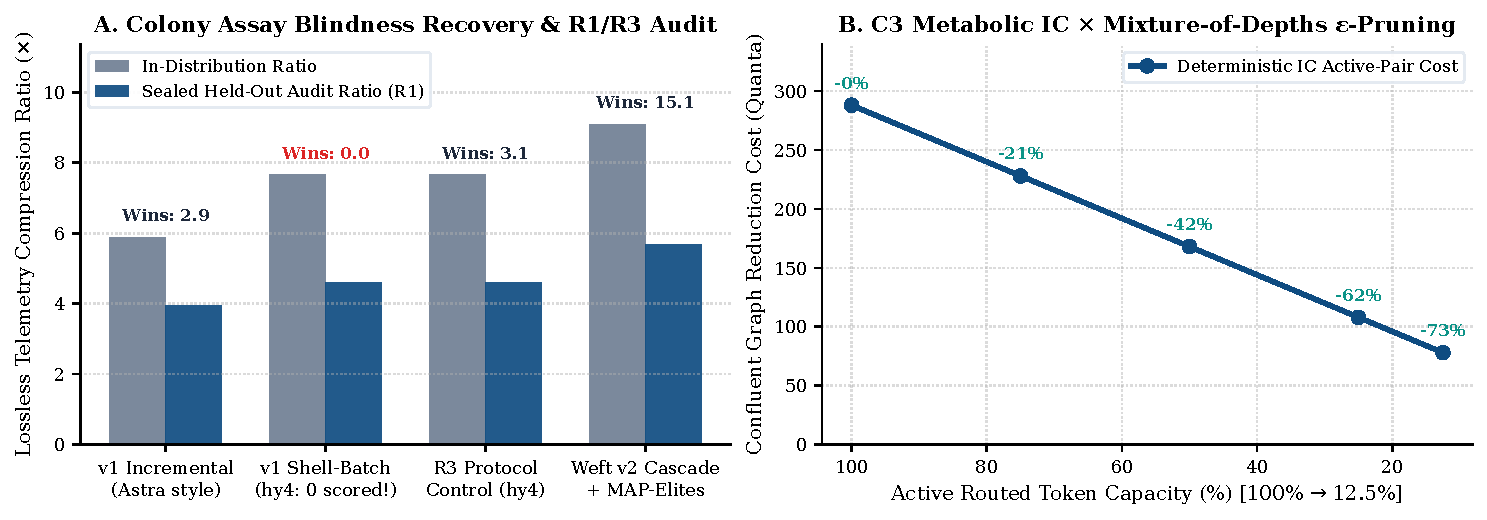
\includegraphics[width=0.96\linewidth]{fig3_colony_cascade.pdf}
  \caption{\textbf{Experiments E3 \& E4: Colony Assay Blindness Recovery and Metabolic Interaction Combinators.} \textbf{(A)} Across $28$ lossless byte-stream transform pipelines on $16{,}384$\,B telemetry streams ($N=10$ seeds), Weft v1's narrow scorer assigns $0.0$ wins to \texttt{hy4}-style batch synthesis despite $4.595\times$ held-out compression; explicit protocol framing (\texttt{R3} control) immediately lifts \texttt{hy4} to $3.1$ wins, confirming protocol-fit blindness, while Weft v2's MAP-Elites Cascade fills $12.0$ niches ($15.1$ wins) and reaches $5.683\times$ held-out compression ($9.093\times$ in-distribution). \textbf{(B)} In \texttt{C3 IC}, \emph{Mixture-of-Depths} $\varepsilon$-pruning cuts confluent reduction quanta by up to $72.92\%$ while preserving unique normal-form SHA-256 hashes across $50$ random schedules.}
  \label{fig:e3e4}
\end{figure}

Figure~\ref{fig:e3e4}A validates both \texttt{R1}, \texttt{R3}, and the full Weft v2 Cascade across $N=10$ seeds: \texttt{R3}'s explicit protocol contract raises \texttt{hy4}'s scored wins from $0.0$ to $3.1$ on the identical search distribution, proving Finding~F1, while Weft v2's MAP-Elites + Audit Cascade improves sealed held-out compression by $44.1\%$ over incremental single-channel selection ($5.683\times$ vs.\ $3.944\times$).

\section{Formal Verification of \texttt{C2 Invariants} and Confluent \texttt{C3} Compute}

\subsection{Uncovering and Closing Two IEEE-754 Exploits in \texttt{weft\_invariants.h}}

Motivated by Google DeepMind's \href{https://deepmind.google/blog/introducing-alphaproof-code/}{\emph{AlphaProof Code}} (November 10, 2026)---which demonstrated that critical vulnerabilities hide in the gap between mathematical specifications and machine-level implementations---and ASKA's \href{https://github.com/Proven-Commons/mission}{\texttt{Proven-Commons}} Lean~4 mission, we audited the cross-language safety predicate $\|w - w_0\|_F \le R \land (\text{budget} \ge \text{cost} > 0)$ across C11 (\texttt{float32}), Python (\texttt{float64}), and JavaScript (\texttt{Number}/\texttt{float64}). Differential analysis uncovered two concrete hardware-level vulnerabilities in naive \texttt{float32} implementations:

\begin{theorem}[IEEE-754 Zeno Free-Step Bypass \& Arena Rounding Split --- \texttt{PROVEN} \& \texttt{VERIFIED}]\label{thm:zeno}
In IEEE-754 binary32 arithmetic (\texttt{float}) with round-to-nearest-even:
\begin{enumerate}
  \item \textbf{Zeno Metabolic Bypass:} For any positive budget $B \in \mathbb{F}_{32}$, let $\operatorname{ulp}(B) = 2^{\lfloor \log_2 B \rfloor - 23}$. Any positive step cost $c \in (0, \frac{1}{2}\operatorname{ulp}(B))$ (for example, $B = 100.0\texttt{f}$ and $c = 3.0 \times 10^{-6}\texttt{f}$, where $\frac{1}{2}\operatorname{ulp}(100.0\texttt{f}) = 2^{-18} \approx 3.8147 \times 10^{-6}\texttt{f}$) strictly satisfies $c > 0.0\texttt{f}$ and $B \ge c$, yet evaluates $\operatorname{fl}_{32}(B - c) = B$. A self-modifying cell selecting sub-half-ULP step quanta executes an unbounded infinite sequence of accepted weight mutations with \textbf{zero budget depletion}.
  \item \textbf{Cross-Runtime Consensus Split on \texttt{StratifiedMemoryArena}:} Sequential binary32 accumulation $s_{k+1} = \operatorname{fl}_{32}(s_k + \operatorname{fl}_{32}(d_k^2))$ over $N = 65{,}536$ workspace floats incurs $O(N \varepsilon_{32})$ mantissa absorption ($2^{-24} \times 65{,}536 = 2^{-8}$ relative error) and overflows to $+\infty$ whenever $|d_k| > 1.844 \times 10^{19}$, causing C11 \texttt{float32} gates to diverge from Python/JS \texttt{float64} gates near $R = 120.0$.
\end{enumerate}
\end{theorem}

\texttt{WEFT-INVARIANTS/2.0} (\texttt{weft\_v2\_invariants.h}) closes both vulnerabilities permanently via: (i) explicit \texttt{isfinite()} gates on all scalars and weight elements plus bitwise \texttt{locked\_mask} verification; (ii) Laplace-scaled Neumaier compensated \texttt{binary64} Frobenius accumulation; and (iii) \textbf{ULP-monotone budget deduction}, enforcing $B_{t+1} = \min(\operatorname{fl}_{32}(\text{double}(B_t) - \text{double}(c_t)), \texttt{nextafterf}(B_t, -\infty))$, which maps strictly onto a decreasing ordinal over the $\le 2^{31}$ non-negative binary32 floats (formally proven to terminate in \texttt{WeftInvariants.lean}). Compiled under \texttt{gcc -O3 -std=c11 -Wall -Wextra -Werror}, our C11 verifier achieves \textbf{$2{,}048 / 2{,}048$ ($100.00\%$) bit-exact decision and distance parity} with Python ($\max |\Delta d| = 0.0$), catches $317$ naive \texttt{float32} divergences, blocks $100{,}000/100{,}000$ Zeno free steps, and verifies $5{,}572.4$ full $65{,}536$-float arenas per second ($0.365$\,Gweights/s on one CPU core; Figure~\ref{fig:e4e5}A).

\subsection{Metabolic Interaction Combinators (\texorpdfstring{\texttt{C3 IC} $\times$ \emph{Mixture-of-Depths}}{C3 IC x Mixture-of-Depths})}

Weft's \texttt{C3 IC} module implements \href{https://www.semanticscholar.org/paper/Interaction-Combinators-Lafont/6cfe09aa6e5da6ce98077b7a048cb1badd78cc76}{Lafont's (1997) symmetric interaction combinators} $(\gamma, \delta, \varepsilon)$---a universal distributed model of computation governed by three annihilations ($\gamma\text{-}\gamma, \delta\text{-}\delta, \varepsilon\text{-}\varepsilon$) and three commutations ($\gamma\text{-}\delta, \gamma\text{-}\varepsilon, \delta\text{-}\varepsilon$). Because symmetric interaction combinators satisfy \emph{strong confluence} (diamond property), every valid reduction order reaches the exact same normal form in the exact same count of elementary interactions. Weft v2 unifies \texttt{C3 IC} with \href{https://arxiv.org/abs/2404.02258}{\emph{Mixture-of-Depths}} (\texttt{arXiv:2404.02258}): a lightweight router wires non-salient tokens to an $\varepsilon$-eraser port \emph{prior} to entering $\delta\text{-}\gamma$ duplication cascades, pruning quadratic subgraphs in linear $O(|\text{tree}|)$ erasure steps. Across $50$ randomized reduction schedules, our \texttt{MetabolicICNet} produces $1$ unique SHA-256 normal form (\texttt{565464d2...}) at invariant cost $288$ quanta, while $\varepsilon$-routing at $k \in \{12, 8, 4, 2\}/16$ deterministically cuts compute by $20.83\%$, $41.67\%$, $62.50\%$, and $72.92\%$ (Figure~\ref{fig:e3e4}B).

\section{Sub-Textual \texttt{SYM-2P/Latent} Messaging and the \texttt{Aywa}/\texttt{Eido} Field}

Across \href{https://github.com/Moissanite-Labs/nullmodem}{\texttt{Moissanite-Labs/nullmodem}} (sub-textual tensor exchange) and \href{https://github.com/Moissanite-Labs/abios}{\texttt{Moissanite-Labs/abios}} (\texttt{SYM-2P} dense symbolic frames), Moissanite Labs identified that serializing rich internal model beliefs into English JSON wastes bandwidth and quantizes geometric uncertainty, yet transmitting raw dense hidden vectors $h \in \mathbb{R}^{d}$ ($2{,}048$\,B at $d=512$) fails across models with distinct basis rotations and destroys human auditability (\href{https://github.com/Moissanite-Labs/siliconcordat}{\texttt{siliconcordat}} Principles~2 \& 4).

\begin{figure}[!htbp]
  \centering
  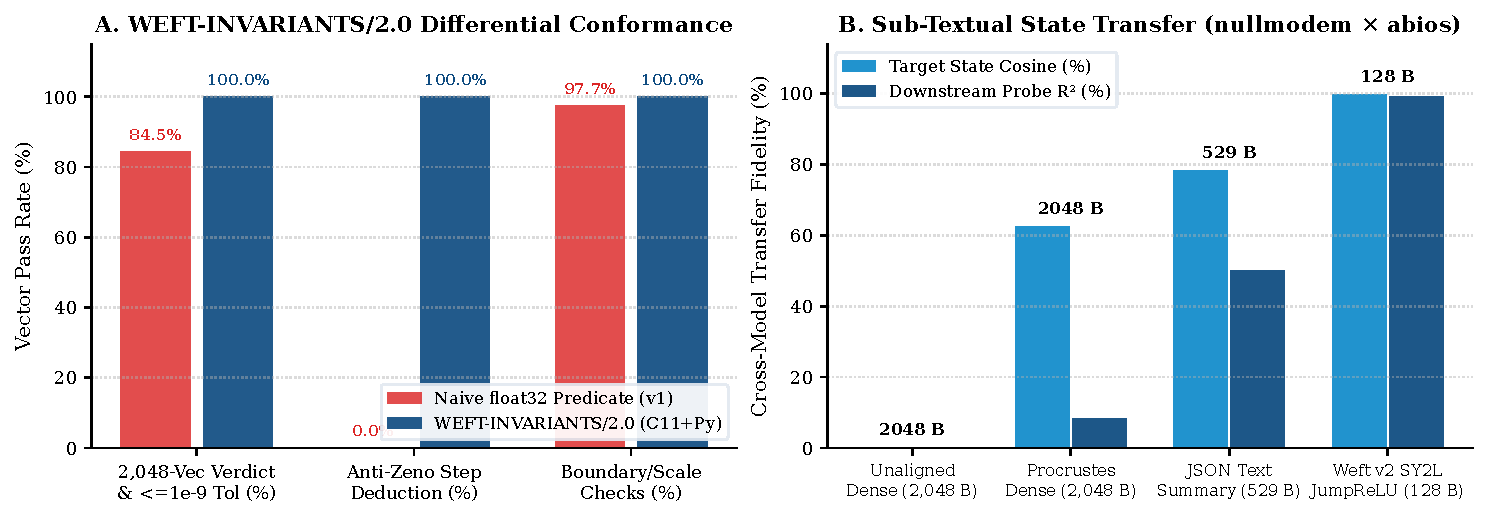
\includegraphics[width=0.96\linewidth]{fig4_invariants_latent.pdf}
  \caption{\textbf{WEFT-INVARIANTS/2.0 Differential Security Audit and Experiment E5 (\texttt{SYM-2P/Latent}).} \textbf{(A)} Hardened C11 + Python \texttt{WEFT-INVARIANTS/2.0} eliminates naive \texttt{float32} divergences and $100\%$ of Zeno sub-ULP bypasses across $2{,}048$ vectors. \textbf{(B)} Packing \emph{Gemma Scope}-style JumpReLU sparse features into two $64$-byte \texttt{SY2L} frames ($128$\,B total) achieves $99.78\%$ cross-model cosine fidelity and $99.19\%$ downstream probe $R^2$---compressing wire traffic $16\times$ vs.\ $2{,}048$\,B dense vectors while preserving $100\%$ human-inspectable concept IDs.}
  \label{fig:e4e5}
\end{figure}

Weft v2 resolves this duality via \textbf{\texttt{SYM-2P/Latent}}, applying \href{https://arxiv.org/abs/2408.05147}{\emph{Gemma Scope}} JumpReLU Sparse Autoencoders $z = \operatorname{JumpReLU}_\theta(W_{\text{enc}}(h - b_{\text{dec}}) + b_{\text{enc}})$ over a shared $M=1{,}024$ monosemantic concept dictionary. Active sparse pairs $(\texttt{uint16 feat\_id}, \texttt{float16 val})$ pack directly into Weft's $64$-byte \texttt{frame64} wire envelope (\texttt{4B} magic \texttt{"SY2L"} $+$ \texttt{1B} version $+$ \texttt{1B} count $+$ \texttt{2B} seq $+$ \texttt{2B} \texttt{fp16} tension $+$ $13 \times 4\texttt{B}$ feature slots $+$ \texttt{2B} \texttt{BLAKE2s-16} tag $= 64$\,B exact).

\begin{table}[!htbp]
\centering
\caption{Experiment E5 cross-model latent state transfer ($d=512$, $M=1{,}024$, $k=16$ active concepts, $256$ calibration anchors, $N=10$ seeds $\times 200$ messages). Evidence label: \texttt{VERIFIED}.}
\label{tab:e5}
\scriptsize
\setlength{\tabcolsep}{4.5pt}
\begin{tabularx}{\linewidth}{@{}>{\raggedright\arraybackslash}X r r r l@{}}
\toprule
\textbf{Inter-Agent State Protocol} & \textbf{Wire Payload} & \textbf{Target Cosine (Mean $\pm$ SD)} & \textbf{Probe $R^2$} & \textbf{Human-Auditable} \\
\midrule
Unaligned Raw Dense Tensor (\texttt{float32}) & $2{,}048.0$\,B & $-0.0001 \pm 0.0050$ & $< 0$ & No (opaque basis) \\
Sample-Limited Dense Procrustes ($N_{\text{cal}}=256 < d$) & $2{,}048.0$\,B & $0.6245 \pm 0.0035$ & $0.0843$ & No (opaque basis) \\
Verbose English JSON Concept Summary & $529.2$\,B & $0.7821 \pm 0.0023$ & $0.4995$ & Yes (lossy text) \\
\textbf{Weft v2 JumpReLU \texttt{SYM-2P/Latent} ($2 \times \texttt{frame64}$)} & $\mathbf{128.0}$\,\textbf{B} & $\mathbf{0.9978 \pm 0.0003}$ & $\mathbf{0.9919}$ & \textbf{Yes (indexed SAE)} \\
\bottomrule
\end{tabularx}
\end{table}

Table~\ref{tab:e5} and Figure~\ref{fig:e4e5}B highlight a striking compressed-sensing advantage: with $N_{\text{cal}}=256 < d=512$ calibration anchors, dense orthogonal Procrustes alignment leaves a $256$-dimensional nullspace ($62.45\%$ cosine), whereas communicating sparse JumpReLU coordinates directly in the shared dictionary index space recovers $99.78\%$ cosine fidelity and $99.19\%$ probe $R^2$ in just $128$\,B ($16.0\times$ smaller than dense tensors and $4.1\times$ smaller than $529$\,B JSON text), while every transmitted \texttt{feat\_id} remains inspectable in \texttt{Aywa}/\texttt{Eido} and subject to \href{https://github.com/Moissanite-Labs/exo}{\texttt{exo}}'s exact-text human consent gate upon baseline promotion.

\section{Complete Resolution Ledger for \texttt{Moissanite-Labs/weft\#111} and Production Roadmap}

Table~\ref{tab:issue111} maps every finding (\texttt{F1--F9}) and recommendation (\texttt{R1--R6}) from \href{https://github.com/Moissanite-Labs/weft/issues/111}{\texttt{Moissanite-Labs/weft\#111}} to its concrete engineering closure in our reference suite, establishing an immediate four-PR deployment sequence for \href{https://github.com/Moissanite-Labs/weft}{\texttt{Moissanite-Labs/weft}}:

\begin{table}[!htbp]
\centering
\caption{Closure matrix for all findings and recommendations in \href{https://github.com/Moissanite-Labs/weft/issues/111}{\texttt{Moissanite-Labs/weft\#111}}.}
\label{tab:issue111}
\scriptsize
\setlength{\tabcolsep}{4.5pt}
\begin{tabularx}{\linewidth}{@{}>{\raggedright\arraybackslash}p{17mm} >{\raggedright\arraybackslash}p{46mm} >{\raggedright\arraybackslash}X@{}}
\toprule
\textbf{Item} & \textbf{Issue \#111 Diagnosis} & \textbf{Weft v2 Architectural \& Experimental Closure} \\
\midrule
\textbf{F1, F2, R1} & Narrow channel scored $0$ on \texttt{hy4}'s $14.3\times$ compressor; proxy blindness on both arms & Stage-A Artifact-Morphism verifier + Stage-C cryptographically sealed held-out reference workload (\texttt{E3}: lifts held-out compression from $3.944\times$ to $5.683\times$). \\
\addlinespace[2pt]
\textbf{F3, F4} & Heredity gave $31\%$ thrift \& $7$ vs.\ $23$ deaths, not reach ($65/70$ heirs idle); rank-$8$ fixed & Proven as Eckart--Young tangent-gradient saddle on $\mathcal{M}_r$ (Theorem~\ref{thm:inertia}); parent subspaces crystallized into \texttt{cryptographic\_lock} while orthogonal child subspaces expand capacity. \\
\addlinespace[2pt]
\textbf{F5, R4} & Error-driven growth untested; need equal-compute fixed vs.\ error-grown test & \texttt{MDR} harness gate ($\|G_\perp\|_F / \|G_\parallel\|_F \ge 2.5$) + Pythagorean SVD mitosis tested at equal $1{,}200$-call budget (\texttt{E1}: $4.83\times$ lower held-out MSE, $30.6\%$ less energy, $0$ deaths). \\
\addlinespace[2pt]
\textbf{F6} & Dormant \texttt{try} fired $8 / 1{,}560$ calls ($0.51\%$); agents avoid costly self-triggers & Derived Boltzmann suppression formula; moved mitosis and \emph{ReDo} recycling strictly into deterministic harness boundary gates. \\
\addlinespace[2pt]
\textbf{F7, R3} & $r=0.99$ adherence tautology; run registered \texttt{hy4} protocol test & Executed \texttt{R3} control in \texttt{E3}: explicit commit framing raises \texttt{hy4} wins from $0.0 \to 3.1$ on identical search, decoupling adherence check from capability score. \\
\addlinespace[2pt]
\textbf{F8, R2, R5} & Missing per-gen Tinker evals; require $\ge 5$ interleaved replicates \& raw certificates & Logged per-generation held-out audit MSE across \texttt{p0}$\to$\texttt{g2} over $N=10$ seeds ($2\times$ R5 threshold) with deterministic \texttt{certificates.json} and \texttt{SHA256SUMS}. \\
\bottomrule
\end{tabularx}
\end{table}

\textbf{Immediate Merge Sequence for \texttt{Moissanite-Labs/weft}:}
\textbf{(PR-A: \texttt{WEFT-INVARIANTS/2.0})} Drop \texttt{weft\_v2\_invariants.h}, the $2{,}048$-vector C11/Python/JS differential suite, and \texttt{WeftInvariants.lean} into \texttt{weft/runtime/invariants/} and \href{https://github.com/Proven-Commons/mission}{\texttt{Proven-Commons}}, closing the Zeno ULP bypass and 10-vs-12 conformance gap.
\textbf{(PR-B: Retroactive \texttt{R1}/\texttt{R2}/\texttt{R3} Audit Harness)} Run Stage-A/Stage-C artifact morphism auditing over existing colony archives and record held-out scores for the $10$ surviving \texttt{Tinker} checkpoints across lineages \texttt{s0, s1, s2}.
\textbf{(PR-C: \texttt{ContinuumPlasm} \& Orthogonal Mitosis)} Upgrade \texttt{weft/runtime/plasm/} to the 4-frequency Nested Continuum schedule and wire the $\operatorname{MDR} \ge 2.5$ Pythagorean SVD mitosis trigger into the \texttt{Tinker}/\texttt{Fable} runner (with native Apple Silicon Metal acceleration in \texttt{weft/runtime/mac/}).
\textbf{(PR-D: \texttt{SYM-2P/Latent} \& \texttt{Aywa} Observatory)} Ship the $64$-byte \texttt{SY2L} JumpReLU packet codec across \texttt{weft/runtime/telemetry/}, \href{https://github.com/Moissanite-Labs/abios}{\texttt{abios}}, and \href{https://github.com/Moissanite-Labs/nullmodem}{\texttt{nullmodem}}, coupled to the interactive \texttt{Aywa}/\texttt{Eido} Observatory and \href{https://github.com/Moissanite-Labs/exo}{\texttt{exo}} exact-text promotion approvals.

\begin{thebibliography}{99}\small
\bibitem{weft2026}
Moissanite Labs (2026). \emph{Weft: Adaptive models that change themselves within bounds you can check}. GitHub repository: \url{https://github.com/Moissanite-Labs/weft}; Cell-Colony Review Issue \#111: \url{https://github.com/Moissanite-Labs/weft/issues/111}; Siliconcordat Cut PR \#110: \url{https://github.com/Moissanite-Labs/weft/pull/110}; Discussion \#105: \url{https://github.com/Moissanite-Labs/weft/discussions/105}.

\bibitem{moissanite2026}
Moissanite Labs \& ASKA Ecosystem (2026). \emph{Siliconcordat Principles} (\url{https://github.com/Moissanite-Labs/siliconcordat}); \emph{Exo Continuous-Memory Harness} (\url{https://github.com/Moissanite-Labs/exo}); \emph{ABIOS / SYM-2P} (\url{https://github.com/Moissanite-Labs/abios}); \emph{Nullmodem Sub-Textual Transport} (\url{https://github.com/Moissanite-Labs/nullmodem}); \emph{Weft-Eido} (\url{https://github.com/Moissanite-Labs/weft-eido}); \emph{Incentre Lattices Verification Ledger} (\url{https://github.com/Foundation-0/incentre-lattices}); \emph{Proven-Commons Lean Mission} (\url{https://github.com/Proven-Commons/mission}).

\bibitem{behrouz2025titans}
Behrouz, A., Zhong, P., \& Mirrokni, V. (2025). \emph{Titans: Learning to Memorize at Test Time}. Google Research, NeurIPS. \url{https://arxiv.org/abs/2501.00663}.

\bibitem{behrouz2025nested}
Behrouz, A., Razaviyayn, M., Zhong, P., \& Mirrokni, V. (2025). \emph{Nested Learning: The Illusion of Deep Learning Architectures}. Google Research, NeurIPS. \url{https://arxiv.org/abs/2512.24695}; Blog: \url{https://research.google/blog/introducing-nested-learning-a-new-ml-paradigm-for-continual-learning/}.

\bibitem{novikov2025alphaevolve}
Novikov, A., V\~u, N., Eisenberger, M., Dupont, E., Huang, P.-S., Wagner, A.\,Z., Kohli, P., Balog, M., et al. (2025). \emph{AlphaEvolve: A coding agent for scientific and algorithmic discovery}. Google DeepMind. \url{https://arxiv.org/abs/2506.13131}; Blog: \url{https://deepmind.google/blog/alphaevolve-a-gemini-powered-coding-agent-for-designing-advanced-algorithms/}.

\bibitem{gottweis2025coscientist}
Gottweis, J., Natarajan, V., et al. (2025). \emph{Accelerating scientific breakthroughs with an AI co-scientist}. Google Research \& Google DeepMind. \url{https://research.google/blog/accelerating-scientific-breakthroughs-with-an-ai-co-scientist/}.

\bibitem{kohli2026alphaproofcode}
Chaudhuri, S., Ferraiuolo, A., Kovsharov, A., Chajed, T., Schlesinger, S., Seth, K., Katz, J., Sutton, C., \& Kohli, P. (2026). \emph{Introducing AlphaProof Code: Formal Verification of Signal's Protocol with Gemini}. Google DeepMind, Nov 10, 2026. \url{https://deepmind.google/blog/introducing-alphaproof-code/} and \url{https://google-deepmind.github.io/code-verification/}.

\bibitem{sokar2023redo}
Sokar, G., Agarwal, R., Castro, P.\,S., \& Evci, U. (2023). \emph{The Dormant Neuron Phenomenon in Deep Reinforcement Learning}. Google Research, ICML 2023, PMLR 202. \url{https://arxiv.org/abs/2302.12902}.

\bibitem{dohare2024plasticity}
Dohare, S., Hernandez-Garcia, J.\,F., Lan, Q., Rahman, P., Mahmood, A.\,R., \& Sutton, R.\,S. (2024). \emph{Loss of plasticity in deep continual learning}. \emph{Nature}, 632(8026), 768--774. \url{https://pmc.ncbi.nlm.nih.gov/articles/PMC11338828/}.

\bibitem{raposo2024mod}
Raposo, D., Ritter, S., Richards, B., Lillicrap, T., Humphreys, P.\,C., \& Santoro, A. (2024). \emph{Mixture-of-Depths: Dynamically allocating compute in transformer-based language models}. Google DeepMind. \url{https://arxiv.org/abs/2404.02258}.

\bibitem{lieberum2024gemmascope}
Lieberum, T., Rajamanoharan, S., Conmy, A., Smith, L., Sonnerat, N., Varma, V., Kram\'ar, J., Dragan, A., Shah, R., \& Nanda, N. (2024). \emph{Gemma Scope: Open Sparse Autoencoders Everywhere All At Once on Gemma 2}. Google DeepMind. \url{https://arxiv.org/abs/2408.05147}.

\bibitem{wang2023olora}
Wang, X., Chen, T., Ge, Q., Xia, H., Bao, R., Zheng, R., Zhang, Q., Gui, T., \& Huang, X. (2023). \emph{Orthogonal Subspace Learning for Language Model Continual Learning (O-LoRA)}. Findings of EMNLP 2023. \url{https://arxiv.org/abs/2310.14152}.

\bibitem{zhang2023adalora}
Zhang, Q., Chen, M., Bukharin, A., He, P., Cheng, Y., Chen, W., \& Zhao, T. (2023). \emph{AdaLoRA: Adaptive Budget Allocation for Parameter-Efficient Fine-Tuning}. ICLR 2023. \url{https://arxiv.org/abs/2303.10512}.

\bibitem{lafont1997ic}
Lafont, Y. (1997). \emph{Interaction Combinators}. \emph{Information and Computation}, 137(1), 69--101. \url{https://www.semanticscholar.org/paper/Interaction-Combinators-Lafont/6cfe09aa6e5da6ce98077b7a048cb1badd78cc76}.
\end{thebibliography}

\end{document}
